\documentclass[aspectratio=169,11pt]{beamer}

\usetheme{metropolis}
\metroset{numbering=fraction,progressbar=frametitle}

\usepackage[T1]{fontenc}
\usepackage{amsmath,amssymb}
\usepackage{booktabs}
\usepackage{tabularx}
\usepackage{listings}
\usepackage{xcolor}
\usepackage{pgfplots}
\pgfplotsset{compat=1.16}
\usepgfplotslibrary{dateplot}

\definecolor{orebg}{HTML}{121214}
\definecolor{oreraised}{HTML}{1A1A1E}
\definecolor{oreoverlay}{HTML}{26262B}
\definecolor{oreline}{HTML}{30363D}
\definecolor{oreink}{HTML}{E3E3E6}
\definecolor{oremuted}{HTML}{A1A1AA}
\definecolor{oreaccent}{HTML}{58A6FF}
\definecolor{oreaccentbright}{HTML}{8AB4F8}
\definecolor{orelogoblue}{HTML}{93B4CD}
\definecolor{oreteal}{HTML}{2DD4BF}
\definecolor{orewarn}{HTML}{D29922}

\colorlet{codebg}{oreraised}
\colorlet{codekw}{oreaccent}
\colorlet{codecm}{oremuted}
\colorlet{codestr}{oreteal}
\colorlet{seriesa}{oreaccent}
\colorlet{seriesb}{orewarn}

\setbeamercolor{normal text}{fg=oreink,bg=orebg}
\setbeamercolor{background canvas}{bg=orebg}
\setbeamercolor{palette primary}{fg=oreink,bg=oreraised}
\setbeamercolor{frametitle}{fg=oreink,bg=oreraised}
\setbeamercolor{alerted text}{fg=oreaccentbright}
\setbeamercolor{progress bar}{fg=oreaccent,bg=oreline}
\setbeamercolor{title separator}{fg=oreaccent,bg=oreline}
\setbeamercolor{block title}{fg=orelogoblue,bg=oreoverlay}
\setbeamercolor{block body}{fg=oreink,bg=oreraised}
\setbeamercolor{block title alerted}{fg=oreaccentbright,bg=oreoverlay}
\setbeamercolor{block body alerted}{fg=oreink,bg=oreraised}
\setbeamercolor{itemize item}{fg=orelogoblue}
\setbeamercolor{enumerate item}{fg=orelogoblue}
\metroset{block=fill}

\graphicspath{{images/}}
\setbeamertemplate{background}{%
  \ifnum\value{page}=1
    \begin{tikzpicture}[remember picture,overlay]
      \node[anchor=north east,inner sep=0pt] at ([xshift=-0.7cm,yshift=-0.5cm]current page.north east)
        {
\includegraphics[height=1.7cm]{ore_studio_wordmark}};
    \end{tikzpicture}%
  \fi
}
\addtobeamertemplate{footline}{}{%
  \nointerlineskip\vbox to 0pt{%
    \begin{tikzpicture}[remember picture,overlay]
      \node[anchor=north east,inner sep=0pt] at ([xshift=-0.3cm,yshift=-0.14cm]current page.north east)
        {
\includegraphics[height=0.72cm]{ore_studio_mark}};
    \end{tikzpicture}%
    \vss}%
}

\pgfplotsset{every axis/.append style={
  axis line style={oremuted},
  tick style={oremuted},
  legend style={fill=none,draw=none,text=oreink}
}}

\lstset{
  language=Python,
  basicstyle=\ttfamily\footnotesize,
  keywordstyle=\color{codekw}\bfseries,
  commentstyle=\color{codecm}\itshape,
  stringstyle=\color{codestr},
  backgroundcolor=\color{codebg},
  columns=fullflexible,
  keepspaces=true,
  showstringspaces=false,
  frame=single,
  framerule=0pt,
  xleftmargin=4pt,
  xrightmargin=4pt,
  upquote=true
}

\newcolumntype{Y}{>{\raggedright\arraybackslash}X}
\newcommand{\code}[1]{\texttt{#1}}

\title{Building Synthetic Market Data Generators}
\subtitle{ORE Studio Market Data Series --- Part 1}
\author{ORE Studio}
\date{}

\begin{document}

\maketitle

\begin{frame}{Agenda}
  \tableofcontents
\end{frame}

\section{The Underlying and the Problem of Market Data}

\begin{frame}{Observing Reality: 6 Months of GBP/USD ``Cable''}
  \begin{columns}[T]
    \begin{column}{0.52\textwidth}
      \centering
      \begin{tikzpicture}
        \begin{axis}[
          date coordinates in=x,
          width=\textwidth, height=5.4cm,
          xmin=2024-01-01, xmax=2024-07-01,
          xtick={2024-01-01,2024-02-01,2024-03-01,2024-04-01,2024-05-01,2024-06-01},
          xticklabels={Jan,Feb,Mar,Apr,May,Jun},
          ylabel={GBP/USD},
          y tick label style={/pgf/number format/.cd,fixed,fixed zerofill,precision=2},
          scaled y ticks=false,
          tick label style={font=\scriptsize}, label style={font=\scriptsize}
        ]
          \addplot[seriesa, thick, no markers] table[col sep=comma,x=date,y=rate] {gbp_usd_2024h1_ecb.csv};
        \end{axis}
      \end{tikzpicture}

      {\scriptsize GBP/USD, Jan--Jun 2024. Daily ECB reference rates via Frankfurter}
    \end{column}
    \begin{column}{0.44\textwidth}
      \small
      Before any code or models, look at real financial data.
      \medskip

      \textbf{What we notice:}
      \begin{itemize}
        \item \textbf{Continuous and bounded:} prices move in smooth, connected trajectories
        \item \textbf{Memory:} today's price level is heavily constrained by yesterday's
        \item \textbf{Regimes:} low volatility alternates with high volatility
      \end{itemize}
    \end{column}
  \end{columns}
\end{frame}

\begin{frame}{Underneath the Chart: The Raw Data Table}
  Every chart is a visual representation of a time-indexed table.
  \bigskip

  \centering
  \begin{tabular}{lll}
    \toprule
    Date ($t_i$) & GBP/USD Spot ($S_i$) & Description \\
    \midrule
    2024-01-02 & 1.2645 & Starting baseline ($S_0$) \\
    2024-01-03 & 1.2628 & Small downward tick \\
    2024-01-04 & 1.2695 & Rebound \\
    \dots & \dots & \emph{126 rows of daily ECB reference rates} \\
    2024-06-28 & 1.2648 & Ending price ($S_N$) \\
    \bottomrule
  \end{tabular}
\end{frame}

\begin{frame}{Defining the Time Series: Software Mapping}
  To a software engineer, this data is a structured array.
  \bigskip

  \centering
  \begin{tabularx}{\textwidth}{llY}
    \toprule
    Math & Software & Meaning in code \\
    \midrule
    $t_i$ & \code{timestamps[i]} & Ordered discrete time steps (e.g.\ daily ECB fixings) \\
    $S_i$ & \code{prices[i]} & The spot price stored at array index \code{i} \\
    $S_0$ & \code{prices[0]} & The starting price of the series \\
    $N$ & \code{len(prices)} & Total observation count (e.g.\ 126 trading days) \\
    \bottomrule
  \end{tabularx}
\end{frame}

\begin{frame}{Why Do We Need Synthetic Data?}
  \textbf{The ORE Studio challenge}
  \begin{itemize}
    \item Risk engines must test thousands of \emph{hypothetical futures} (Monte Carlo scenarios) to calculate potential future exposure and risk metrics
    \item Real historical data for every possible future scenario is restricted, expensive or non-existent
  \end{itemize}
  \bigskip

  \begin{alertblock}{Our mission}
    Generate realistic artificial time series that mimic the statistical properties of the real GBP/USD chart.
  \end{alertblock}
\end{frame}

\section{A Trivial Stochastic Process: The Uniform Random Walk}

\begin{frame}{What is a Stochastic Process?}
  \textbf{The intuition}
  \begin{itemize}
    \item A deterministic process always gives the same output for a given input (e.g.\ $y = 2x$)
    \item A \alert{stochastic process} is a sequence of random variables indexed over time
  \end{itemize}
  \bigskip

  \textbf{The software engineer's definition}

  A loop over an array. Each step appends a value from a random number generator:
  \[
    \text{prices}[i] = \text{prices}[i-1] + \text{RNG}()
  \]
\end{frame}

\begin{frame}{Sampling from a Uniform Distribution}
  \textbf{The simplest RNG:} in $U(a, b)$, every value between $a$ and $b$ has equal probability.
  \bigskip

  \textbf{Our first trivial model}
  \begin{itemize}
    \item Daily moves $\Delta S_i = S_i - S_{i-1}$ come from a uniform distribution:
    \[
      \Delta S_i \sim U(-0.0081,\, +0.0081)
    \]
    \item State update:
    \[
      S_i = S_{i-1} + \Delta S_i
    \]
  \end{itemize}
\end{frame}

\begin{frame}[fragile]{Code: Uniform Random Walk}
\begin{lstlisting}
import numpy as np
import pandas as pd

np.random.seed(42)
N = 126             # 6 months (~126 trading days)
S0 = 1.2645         # Initial GBP/USD spot price
step_bound = 0.0081 # Uniform bounds [-0.0081, +0.0081]

delta_S = np.random.uniform(low=-step_bound, high=step_bound, size=N - 1)
prices = np.zeros(N)
prices[0] = S0
prices[1:] = S0 + np.cumsum(delta_S)
\end{lstlisting}
\end{frame}

\begin{frame}{Why the Eye Test Is Not Enough}
  \begin{columns}[T]
    \begin{column}{0.56\textwidth}
      \centering
      \pgfmathsetseed{42}
      \xdef\walkspot{1.2645}
      \xdef\walkpoints{(0,1.2645)}
      \foreach \i in {1,...,125} {
        \pgfmathsetmacro{\nextspot}{\walkspot + 0.0081*rand}
        \xdef\walkspot{\nextspot}
        \xdef\walkpoints{\walkpoints (\i,\walkspot)}
      }
      \begin{tikzpicture}
        \begin{axis}[
          width=\textwidth, height=5.4cm,
          xlabel={Trading day $i$}, ylabel={$S_i$},
          xmin=0, xmax=125,
          y tick label style={/pgf/number format/.cd,fixed,fixed zerofill,precision=2},
          scaled y ticks=false,
          tick label style={font=\scriptsize}, label style={font=\scriptsize}
        ]
          \addplot[seriesa, thin, no markers] coordinates {\walkpoints};
        \end{axis}
      \end{tikzpicture}

      {\scriptsize One uniform walk: $N=126$, $S_0=1.2645$, drawn by LaTeX at build time, not NumPy's seed 42}
    \end{column}
    \begin{column}{0.40\textwidth}
      \textbf{Visual observation}

      With its volatility matched to GBP/USD, the path looks plausible. Real and synthetic are hard to tell apart by eye.
      \bigskip

      \textbf{The engineering problem}

      The model still has hard step bounds and no fat tails. ``Looks right'' cannot be a software assertion. We need \alert{numeric, quantitative metrics}.
    \end{column}
  \end{columns}
\end{frame}

\section{Measurements, Deviations and Log Returns}

\begin{frame}{The Flaw of Raw Price Differences}
  Raw differences $S_t - S_{t-1}$ measure absolute price movement.
  \bigskip

  \centering
  \begin{tabular}{rrr}
    \toprule
    Move & Asset price & Relative size \\
    \midrule
    \$1.00 & \$10.00 & 10\% (massive) \\
    \$1.00 & \$10{,}000 & 0.01\% (trivial) \\
    \bottomrule
  \end{tabular}
  \bigskip

  \raggedright
  \alert{The flaw:} raw deviations depend entirely on the absolute price level.
\end{frame}

\begin{frame}{Measuring Spread: The Cancellation Problem}
  To see how spread out the data is, start with the distance of each return from the mean: $(r_i - \mu)$.
  \bigskip

  The mean is the exact centre. Positive and negative deviations \alert{cancel exactly to zero}:
  \[
    \sum_{i=1}^{N} (r_i - \mu) = 0
  \]
\end{frame}

\begin{frame}{Fixing Sign Cancellation: Why Standard Deviation?}
  \begin{columns}[T]
    \begin{column}{0.58\textwidth}
      \small
      \textbf{Option A: absolute deviations} $|r_i - \mu|$

      Intuitive, but $|x|$ is not differentiable at $x=0$. This breaks calculus and optimisation.
      \medskip

      \textbf{Option B: squared deviations} $(r_i - \mu)^2$

      Removes negative signs, is smooth and differentiable, and heavily penalises extreme shocks.
      \medskip

      \textbf{Square root:} restores the units of the data.
      \[
        \sigma = \sqrt{\frac{1}{N-1} \sum_{i=1}^{N} (r_i - \mu)^2}
      \]
    \end{column}
    \begin{column}{0.38\textwidth}
      \centering
      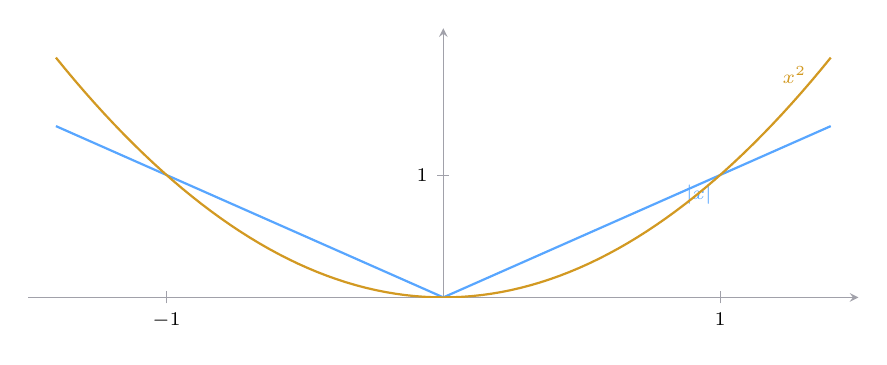
\begin{tikzpicture}
        \begin{axis}[
          width=\textwidth, height=5cm,
          axis lines=middle, xmin=-1.5, xmax=1.5, ymin=0, ymax=2.2,
          xtick={-1,1}, ytick={1},
          tick label style={font=\scriptsize},
          domain=-1.4:1.4, samples=81, no markers
        ]
          \addplot[seriesa, thick] {abs(x)} node[pos=0.8,right,font=\scriptsize] {$|x|$};
          \addplot[seriesb, thick] {x^2} node[pos=0.97,left,font=\scriptsize] {$x^2$};
        \end{axis}
      \end{tikzpicture}
    \end{column}
  \end{columns}
\end{frame}

\begin{frame}{Moving to Returns: Prices are Multiplicative}
  \small
  From 1.20 to 1.26, GBP/USD did not add 0.06 like a counter. It \alert{scaled up by 5\%}: $1.20 \times 1.05 = 1.26$.
  \medskip

  \textbf{Step 1: simple percentage returns}
  \[
    R_t = \frac{S_t - S_{t-1}}{S_{t-1}} = \frac{S_t}{S_{t-1}} - 1
  \]

  \textbf{Limitations in software}
  \begin{itemize}
    \item \textbf{Asymmetry trap:} a 50\% drop ($100 \rightarrow 50$) needs a +100\% gain ($50 \rightarrow 100$) to recover. This breaks symmetric assumptions.
    \item \textbf{Multiplicative chains:} compounding requires multiplication loops, which bring numerical drift and awkward window calculations:
    \[
      (1 + R_{\text{total}}) = (1 + R_1) \times (1 + R_2) \times \dots \times (1 + R_N)
    \]
  \end{itemize}
\end{frame}

\begin{frame}{Step 2: Why Log Returns Solve Engineering Problems}
  \small
  Logarithms convert multiplication into addition: $\ln(A \times B) = \ln(A) + \ln(B)$.
  \[
    r_t = \ln\left(\frac{S_t}{S_{t-1}}\right) = \ln(S_t) - \ln(S_{t-1})
  \]

  \begin{enumerate}
    \item \textbf{Time additivity:} the total return over $N$ steps is a vector sum, $r_{\text{total}} = \sum_{i=1}^{N} r_i$ (\code{np.sum()})
    \item \textbf{Symmetry around zero:} drops and gains are symmetric in log space, a clean fit for Gaussian distributions
    \item \textbf{Non-negativity guarantee:} reconstruction uses exponentiation, $S_t = S_0 e^{\sum r_i}$, so prices never fall below zero. The Euler--Maruyama scheme later in this deck has no such guarantee.
  \end{enumerate}
\end{frame}

\begin{frame}[fragile]{Code: Measuring and Reconstructing Prices}
\begin{lstlisting}
import numpy as np
# Continues the walk code: uses its prices array
# 1. Compute log returns array from price array: ln(S_t / S_{t-1})
log_returns = np.log(prices[1:] / prices[:-1])

# 2. Compute basic statistical parameters
mean_return = np.mean(log_returns)
volatility = np.std(log_returns, ddof=1)
print(f"Mean Daily Return (mu): {mean_return:.6f}")
print(f"Daily Volatility (sigma): {volatility:.6f}")

# 3. Reconstruct prices array from log returns via cumsum + exp
S0 = 1.2645
reconstructed_prices = S0 * np.exp(np.cumsum(np.insert(log_returns, 0, 0)))
\end{lstlisting}
\end{frame}

\section{Discrete vs.\ Continuous Time and Space}

\begin{frame}{The Developer's Dilemma: Math vs.\ CPU}
  \textbf{The math textbook (continuous world)}

  Stochastic calculus defines $S_t$ and $W_t$ for \emph{every} real $t \ge 0$. You can zoom in infinitely between $t = 1.0$ and $t = 1.0001$.
  \medskip

  \textbf{The CPU and RAM (discrete world)}

  Memory consists of finite arrays (\code{std::vector<double>} or NumPy arrays) indexed by integers $i = 0, 1, 2, \dots, N$.
  \medskip

  \alert{The bridge:} we \textbf{discretize} the equations and slice continuous time into finite steps $\Delta t$.
\end{frame}

\begin{frame}{Mental Model: Video Game Frames vs.\ Analog Motion}
  \footnotesize
  \begin{tabularx}{\textwidth}{>{\bfseries}l Y Y}
    \toprule
    Concept & Continuous reality (math) & Discrete implementation (code) \\
    \midrule
    Analogy & A car on a highway, covering infinite points on the road & A video game at 60 FPS, updating the position every $\frac{1}{60}$ s \\
    Time variable & $t \in \mathbb{R}$ & Array index \code{i} (\code{t = i * dt}) \\
    State evaluation & Can evaluate $S(t)$ at $t = 1.23456789\dots$ & Can only look up \code{prices[i]} at exact indices \\
    Random shocks & Brownian motion $W_t$ (unbroken random path) & A draw $Z \sim \mathcal{N}(0,1)$ at each discrete tick \\
    \bottomrule
  \end{tabularx}
  \bigskip

  \begin{block}{The core rule}
    We use continuous-time calculus to derive the rules of motion. We always implement them as discrete recurrence relations in a \code{for} loop.
  \end{block}
\end{frame}

\begin{frame}{Translating Continuous Equations into Discrete Code}
  \textbf{Continuous form (stochastic differential equation)}
  \[
    dS_t = \mu S_t\, dt + \sigma S_t\, dW_t
  \]
  {\small $dt$ is an infinitesimally small time step. $dW_t$ is a continuous Wiener increment.}
  \bigskip

  \textbf{Discrete approximation (Euler--Maruyama)}

  {\small Replace $dt$ with $\Delta t$ (e.g.\ $1/252$ for a daily step). Replace $dW_t$ with a normal draw scaled by $\sqrt{\Delta t}$:}
  \[
    S_{i} = S_{i-1} + \mu S_{i-1} \Delta t + \sigma S_{i-1} \sqrt{\Delta t}\, Z_i, \quad Z_i \sim \mathcal{N}(0, 1)
  \]
\end{frame}

\begin{frame}[fragile]{Code: Discretization Parameters}
\begin{lstlisting}
import numpy as np

T = 0.5             # Total time horizon (0.5 years ~ 6 months)
N = 126             # Number of discrete steps (trading days)
dt = T / N          # Size of each discrete time step (Delta t)
S0 = 1.2645         # Initial spot price
mu = 0.0005         # Annual drift
sigma = 0.059       # Annual volatility

prices = np.zeros(N)
prices[0] = S0
\end{lstlisting}
\end{frame}

\begin{frame}[fragile]{Code: The Euler--Maruyama Update Loop}
\begin{lstlisting}
for i in range(1, N):
    Z = np.random.normal(0.0, 1.0)
    # Euler-Maruyama discrete update step
    dS = mu * prices[i-1] * dt + sigma * prices[i-1] * np.sqrt(dt) * Z
    prices[i] = prices[i-1] + dS

print("First 5 discrete price points:", prices[:5])
\end{lstlisting}
\end{frame}

\section{Normal Distributions, Wiener Processes and Brownian Motion}

\begin{frame}{The Shape of Reality: The Normal Distribution}
  \textbf{What real data shows}

  A histogram of real GBP/USD log returns forms a bell curve. Small changes happen constantly. Extreme changes happen rarely.
  \bigskip

  \textbf{Gaussian definition}

  Defined by mean $\mu$ and variance $\sigma^2$:
  \[
    r_t \sim \mathcal{N}(\mu, \sigma^2)
  \]
\end{frame}

\begin{frame}{Gaussian vs.\ Uniform: Why It Matters}
  \begin{columns}[T]
    \begin{column}{0.52\textwidth}
      \small
      \begin{tabularx}{\textwidth}{>{\bfseries}l Y Y}
        \toprule
        & $U(a, b)$ & $\mathcal{N}(\mu, \sigma^2)$ \\
        \midrule
        Bounds & Hard cutoffs: impossible outside $[a, b]$ & Infinite tails: any value is possible, though rare \\
        \addlinespace
        Clustering & Every value in the range is equally likely & Values cluster heavily around $\mu$ \\
        \bottomrule
      \end{tabularx}
    \end{column}
    \begin{column}{0.44\textwidth}
      \centering
      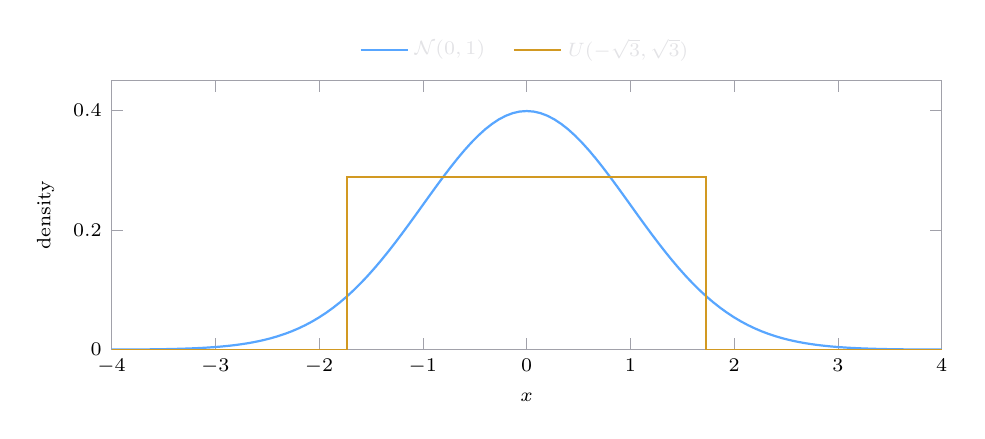
\begin{tikzpicture}
        \begin{axis}[
          width=\textwidth, height=5cm,
          xmin=-4, xmax=4, ymin=0, ymax=0.45,
          xlabel={$x$}, ylabel={density},
          tick label style={font=\scriptsize}, label style={font=\scriptsize},
          y tick label style={/pgf/number format/.cd,fixed,precision=1},
          legend style={font=\scriptsize,draw=none,at={(0.5,1.03)},anchor=south,legend columns=2,/tikz/every even column/.append style={column sep=8pt}},
          legend cell align=left
        ]
          \addplot[seriesa, thick, no markers, domain=-4:4, samples=121]
            {exp(-x^2/2)/sqrt(2*pi)};
          \addlegendentry{$\mathcal{N}(0,1)$}
          \addplot[seriesb, thick, no markers] coordinates
            {(-4,0) (-1.732,0) (-1.732,0.2887) (1.732,0.2887) (1.732,0) (4,0)};
          \addlegendentry{$U(-\sqrt{3},\sqrt{3})$}
        \end{axis}
      \end{tikzpicture}

      {\scriptsize Both have variance 1}
    \end{column}
  \end{columns}
\end{frame}

\begin{frame}[fragile]{Code: Upgrading to a Normal Random Walk}
\begin{lstlisting}[basicstyle=\ttfamily\scriptsize]
import numpy as np

mu = 0.000002  # Daily drift
sigma = 0.0037 # Daily volatility
N = 126

# 1. Draw standard normal random variables
Z = np.random.normal(loc=0.0, scale=1.0, size=N - 1)

# 2. Scale by volatility and add drift
log_returns = mu + sigma * Z

# 3. Reconstruct prices: S_t = S_{0} * exp(cumsum(log_returns))
prices = np.zeros(N)
prices[0] = 1.2645
prices[1:] = prices[0] * np.exp(np.cumsum(log_returns))
\end{lstlisting}
\end{frame}

\begin{frame}{Continuous Time: Wiener Processes and Brownian Motion}
  \textbf{The Wiener process $W_t$}: the continuous-time foundation of quantitative finance.
  \bigskip

  Over an interval $\Delta t$, the change $\Delta W$ is normal with mean 0 and variance $\Delta t$:
  \[
    \Delta W = \sqrt{\Delta t} \cdot Z \sim \mathcal{N}(0, \Delta t), \quad Z \sim \mathcal{N}(0, 1)
  \]

  \begin{alertblock}{The bridge to Part 2}
    The $\sqrt{\Delta t}$ scaling rule makes volatility scale correctly across daily, hourly or sub-second ticks. This sets up stochastic differential equations such as Geometric Brownian Motion.
  \end{alertblock}
\end{frame}

\end{document}
